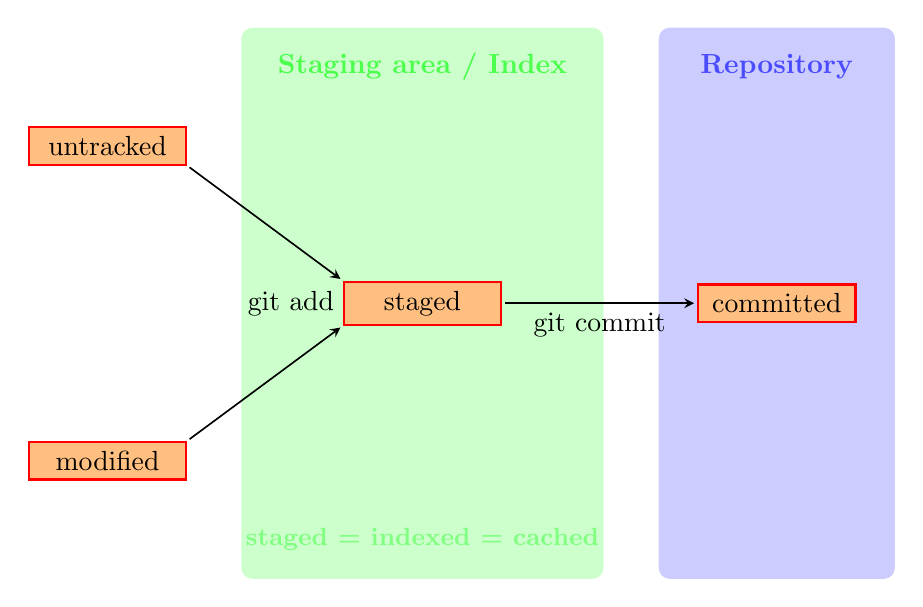
\begin{tikzpicture}
[
gitstate/.style={rectangle, minimum width=2cm, fill=orange!50, draw=red, thick},
link/.style={->, shorten <=1pt, shorten >=1pt, >=stealth, semithick},
label/.style={black}
]

\fill [green!20, rounded corners] (-2.3,-3.5) rectangle (2.3,3.5);
\node[text=green!70] at (0,3) {\textbf{Staging area / Index}};
\node[text=green!50] at (0,-3) {\textbf{\small staged = indexed = cached}};
\fill [blue!20, rounded corners] (3,-3.5) rectangle (6,3.5);
\node[text=blue!70] at (4.5,3) {\textbf{Repository}};

% file states 
\node at (-4, 2) [gitstate] (untracked) { untracked };
\node at (-4, -2) [gitstate] (modified) { modified };
\node at (0, 0) [gitstate] (staged) { staged };
\node[left] at (-1,0) {\hlcommand{git add}};

\node at (4.5, 0) [gitstate] (committed) { committed };

% links between the states
\draw [link] (untracked.south east) to (staged.north west);
\draw [link] (modified.north east) to (staged.south west);
\draw [link] (staged) to node [label,auto,swap] {\hlcommand{git commit}} (committed);

\end{tikzpicture}
